\section{Обзор литературы}

\section{Ключевые понятия и термины}

\TODO: нет такой главы, это всё по другим главам расползётся

\subsection{Основные понятия из теории формальных языков}



\begin{definition}[Конечный автомат (?)]
    НКА и ДКА
    
\end{definition}

\begin{definition}[Рекурсивный конечный автомат (РКА)]
    \textit{Для простоты тут будет немного не такое определение, как в~\cite{Alur05}}

    Это набор компонент $M_1, M_2, \dots , M_k$, где каждая компонента $M_i$~--- это пятёрка $\langle Q_i, \Sigma_i, En_i, Ex_1, \delta_i \rangle$, где 
        \begin{itemize}
          \setlength\itemsep{-0.1em}
          \item $Q_i$~--- конечное множество состояний
          \item $\Sigma_i$~--- конечный алфавит
          \item $En_i \subset Q_i$~--- множество начальных состояний
          \item $Ex_i \subset Q_i$~--- множество конечных состояний
          \item $\delta_i \colon Q_i \times (\Sigma_i \cup \bigcup\limits_{j = 1}^k En_i \times Ex_i ) \to Q_i$~--- функция перехода. У $\delta_i$ есть два типа переходов: \textit{внутренние}, которые работают как обычные переходы в НКА и \textit{рекурсивные}, которые делают вызов другой компоненты (при этом обозначая начальную и конечную вершину в ней).
        \end{itemize}

    Неформально, это набор компонент, каждая из которых представляет собой ДКА, на рёбрах которого могут быть ``рекурсивные вызовы'' других компонент.

    \TODO: картинка с примером
    
\end{definition}

\begin{definition}[Прямое произведение автоматов]

\TODO

\end{definition}

\subsection{Постановка задачи}

\subsubsection{Всякие специфичные для задачи штуки}

\begin{definition}[Транзитивное замыкание]

\TODO

\end{definition}

\begin{definition}[Инкрементальное транзитивное замыкание]

\TODO

\end{definition}


\subsubsection{Просто определения, я не придумала, как это что это как его называть}

\begin{definition}[Система Непересекающихся Множеств (СНМ)]
    \TODO
\end{definition}


\TODO: \textit{Это всё будет красиво ужато в абзацы, а не останется в виде списка}

\subsection{Решения задачи в общем случае}

\begin{enumerate}
    \item $\O(n^3 k^3)$ \cite{Reps97}

    Грамматика приводится к Нормальной форме Хомского, считается $dp_{i,j,c}$~--- выводится ли путь $i \path j$ из нетерминала $s$, при добавлении 1 ($dp_{i,j,A} = 1$) перебираются все соседние нетерминалы $B$, т.ч. $\exists C \to AB$ (или $C \to BA$) и $k \in V(G)$, и если $dp_{j, k, B}$ (или $dp_{k, i, B}$), то $dp_{i, k, C} = 1$ (или $dp_{k, j, C} = 1$) и $(i, k, C)$ добавляется в рабочую очередь.

    \item $\O(n^3 k^3 / \log n)$ \cite{Chaudhuri08}

    Алгоритм \cite{Reps97}, к которому применили метод 4 русских

\end{enumerate}

\TODO: Написать про BMM-сложность.

\subsection{Решения задачи в частных случаях}

Понятно, что для решения практических задач далеко не всегда нужна CFPQ в общем случае. Чаще всего для каждой конкретной задачи нужна конкретная КС грамматика, а иногда ещё и понятны ограничения на тип графа.

Пользуясь этой информацией (ограничениями на тип грамматики и графа) можно конструировать частные и потому более быстрые решения. Этим уже занимались, сейчас мы выпишем всё, что на текущий момент известно:

\begin{enumerate}
    \item Язык Дика $\O(n^3 k)$ \cite{Kodumal04}

    Просто применить алгоритм Репса \cite{Reps97} и нормально оценить время работы.

    \item Язык Дика (почти) $\O(n^3)$ \cite{Rehof01}

    Ещё более точный анализ алгоритм Репса \cite{Reps97}, учитывающий, что построенный (для конкретного анализа) граф содержит константное число скобок

    \item Язык Дика на одном типе скобок $D_1$ $\O(n^{\omega} \log^2 n)$ \cite{Mathiasen21}

    Ищем bell-shaped пути: удваиваем рёбра, ищем пути с серединкой из bell-shaped пути поменьше (так $\log n^2$ раз).

    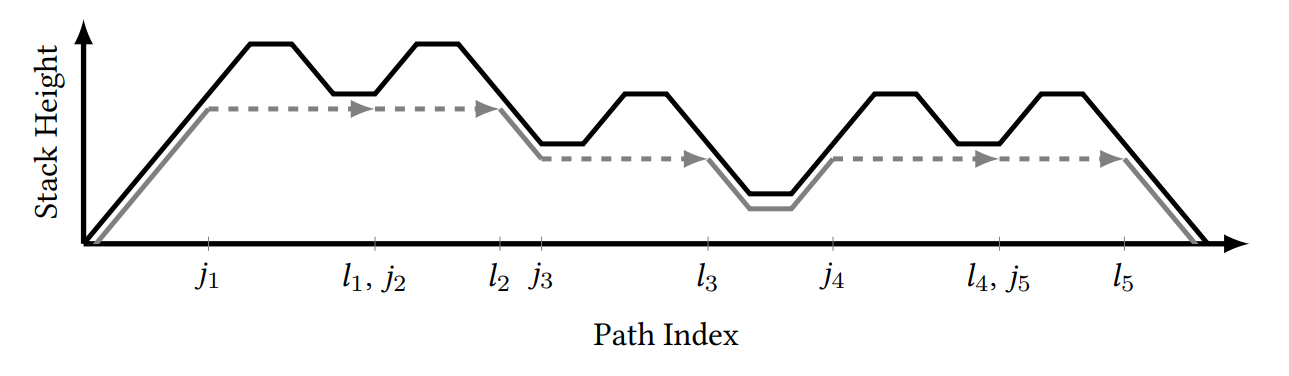
\includegraphics[width=0.75\linewidth]{img/dyck1_path.png}

    Сжимаем bell-shaped пути в $\eps$-рёбра. Снова ищем и снова сжимаем. После каждого сжимания мы убираем все локальные максимумы. Чем больше был максимум, тем длиннее $\eps$-ребро. Хуже всего, когда все новые рёбра длины 2. В любом случае путь становится короче хотя бы в 2 раза, так что таких итераций потребуется не более $\log n^2$ (есть лемма, что найдётся путь длины не более $\O(n^2)$). 

    \item Двунаправленные графы и язык Дика

    Существует несколько частных решений для задачи Диковой достижимости на двунаправленных графах:

    \begin{itemize}
        \item Деревья \cite{Yuan09}

        $\O(n \log n \log k)$~--- центроиды + внутри что-то идейное

        \item Общий случай \cite{Chatterjee17}

        Решение основано на двух фактах. Первый: в двунаправленном графе формируются компоненты Диковой достижимости. Второй: если есть две вершины $u, v$ и компонента Диковой достижимости $C$, такие что $u \xrightarrow{\alpha_i} C$ и $v \xrightarrow{\alpha_i} C$, то $u$ и $v$ тоже лежат в одной компоненте Диковой достижимости. 

        Пользуясь этими фактами, алгоритм с помощью СНМ'а поддерживает компоненты Диковой достижимости и исходящие из них рёбра, чтобы быстро искать новые пары вершин, принадлежащих одной компоненте.

        Итоговая асимптотика алгоритма $\O(m + n \alpha(n))$.
    \end{itemize}

    \item Interleaved Dyck-reachability

        Алгоритм за $\O(n^7)$ для $D_1 \bigodot D_1$ достижимости на bidirected графах~\cite{Li21}

        \textit{Там $\O(n^7)$, потому что авторы~--- дурачки, не умеют рёбра в графе посчитать}

        \textit{Ну или я дурачок, там одно из двух}

        \textit{Было ещё про это (там, вроде, про один из языков сказали, что он bounded, поэтому можно пересекать с регулярным): 
        \url{https://dl.acm.org/doi/pdf/10.1145/3296979.3192378}}
        \TODO: \textit{надо прочитать, что там пишут...}

    \item Граф-цепочка $\O(n^{\omega})$ \cite{Valiant1975}

        CFPQ на графе-цепочке~--- просто задача КС-распознавания (CF-recognition). А она решается за перемножение булевых матриц \cite{Valiant1975}

    \item Ацикличный граф $\O(n^{\omega})$ \cite{Yannakakis1990}

        Ацикличный граф~--- это почти бамбук (= цепочка), нужно только его потопсорить (и где-то ещё быть аккуратным, я не совсем помню сведение)

    \item Bounded-stack RSM $\O(n^3 k^3 / \log^2)$ \cite{Chaudhuri08}

        RSM, который не уходит в рекурсию (т.е. есть из конца ребра $\xrightarrow{S}$ не достижимо никакое ребро $\xrightarrow{S}$)

        Тут применяется какое-то более хитрое (я ещё не разбиралась) итеративное транзитивное замыкание (что-то с dfs'ом, а потом ещё 4 русских сверху, кажется)

    \item Hierarchical FSM $\O(n^{\omega} k^{\omega})$ \cite{Chaudhuri08}

        RSM, в котором боксы упорядочены (топсорт) и бокс с меньшим номером содержит рёбра только с вызовами боксов с большим номером. Задают регулярный язык, но размер FSM может быть экспоненциальным относительно размера RSM.

        Алгоритм идёт в порядке, обратном топсорту, и считает транзитивное замыкание внутри бокса, чтобы провести все рёбра, которые ему соответствуют.

\end{enumerate}

% \subsection{Приложения}

% \textit{Эта часть не для диплома, а для души, потом она в сжатом виде переедет в introduction}

% \begin{itemize}

%     \item Базы данных

%     Querying and storing large volumes of data is an ever-actual concern in computing. Relational databases have been successfully used by the database community and achieved great maturity over the last 40 years [6, 11]. The success of the relational database model relies on a well structured data representation and management, as well as on the use of a (very intuitive and widely used) declarative query language.

%     \item Статический анализ



% \end{itemize}


\subsection{Выводы и результаты по главе}

\TODO